% =============================================================================
% Futebole: methodology paper for the repository soccer simulation engine.
% Regenerate inputs:
%   venv/bin/python experiments/run_experiments.py
%   venv/bin/python experiments/aggregate.py
% Build: (cd paper && TEXMFHOME=texmf pdflatex main.tex)
% =============================================================================
\documentclass[10pt,twocolumn]{article}

\usepackage[margin=1.9cm,columnsep=0.7cm]{geometry}
\usepackage{mathptmx}
\usepackage{courier}
\usepackage[T1]{fontenc}
\usepackage[utf8]{inputenc}
\usepackage{microtype}
\usepackage{amsmath,amssymb}
\usepackage{graphicx}
\usepackage{booktabs}
\usepackage{multirow}
\usepackage{threeparttable}
\usepackage{caption}
\usepackage{subcaption}
\usepackage{siunitx}
\usepackage{xcolor}
\usepackage{tikz}
\usetikzlibrary{arrows.meta,positioning,shapes.geometric,calc,fit}
\usepackage{pgfplots}
\pgfplotsset{compat=1.18}
\usepackage{algorithm}
\usepackage{algpseudocode}
\usepackage[hidelinks]{hyperref}
\usepackage[capitalise,noabbrev]{cleveref}

\graphicspath{{figures/}}

% Generated results (row macros; regenerated by experiments/aggregate.py).
\input{generated/summary_main}
\input{generated/summary_flow}
\input{generated/pvalues}

\definecolor{barblue}{RGB}{70,110,170}
\definecolor{basered}{RGB}{190,60,50}
\definecolor{boxgray}{RGB}{245,245,245}

\captionsetup{font=small,labelfont=bf}

% Relax float placement so results tables/plots stay near their section.
\setcounter{topnumber}{3}
\setcounter{dbltopnumber}{3}
\setcounter{totalnumber}{6}
\renewcommand{\topfraction}{0.95}
\renewcommand{\dbltopfraction}{0.95}
\renewcommand{\textfraction}{0.05}
\renewcommand{\floatpagefraction}{0.85}
\renewcommand{\dblfloatpagefraction}{0.85}

\newcommand{\px}{\ensuremath{\,\mathrm{px}}}
\newcommand{\pxs}{\ensuremath{\,\mathrm{px/s}}}
\newcommand{\code}[1]{\texttt{#1}}

\tikzset{
  block/.style={rectangle, rounded corners=2pt, draw=black!70, fill=boxgray,
                minimum height=5.5mm, minimum width=2.1cm, align=center,
                font=\scriptsize, inner sep=2pt},
  decision/.style={diamond, aspect=2.4, draw=black!70, fill=boxgray,
                   align=center, font=\scriptsize, inner sep=1pt},
  state/.style={circle, draw=black!70, fill=boxgray, minimum size=1.25cm,
                align=center, font=\scriptsize},
  arrow/.style={-{Stealth[length=2mm]}, thick, black!70},
  lbl/.style={font=\scriptsize, align=center},
}

\title{\vspace{-4mm}\textbf{Futebole: An Agent-Based 2D Soccer Simulation Engine with
Role-Aware Tactics and Mixed Human/AI Control --- Methodology and a
Parametric Self-Evaluation}\vspace{-1mm}}

\author{%
Marcos Teixeira\\[1mm]
\small \textit{Futebole Project, v0.2.0}\\
\small \today
}
\date{}

\begin{document}

\twocolumn[
\begin{@twocolumnfalse}
\maketitle
\vspace{-6mm}
\begin{abstract}
\noindent
This paper documents the methodology of \emph{Futebole}, an open,
lightweight two-dimensional soccer simulation with two execution modes:
reproducible all-AI matches between teams of six agents (five outfield
players and a goalkeeper), and interactive mixed-control matches in which a
human steers one selected player while the team AI coordinates the remaining
five. The engine couples (i)~timestep-aware point-mass physics with
exponential rolling friction, capped kick speeds and
distance-scaled kick power; (ii)~an order-independent probabilistic
possession contest with tackles, fouls and dead-ball restarts (throw-ins,
corners, goal kicks, kickoffs) and a simplified offside law; and (iii)~a
layered team-behaviour model comprising a three-state team machine, elastic
formations, a two-bank defensive block, goal-side man-marking, rest defence,
lane-aware decision passing, angle-gated shooting with distance-scaled aim
noise, and a dedicated goalkeeper policy. The interactive path adds semantic,
rebindable input, phase-aware player selection, sprint/pass/shoot actions and
an explicit exclusion boundary between human and AI commands, while retaining
the same physics, cooldowns and central possession rules. Every mechanism is
specified with its governing equations and algorithms, and is illustrated
with screenshots taken directly from the running simulation. We evaluate the
all-AI mode exclusively through \emph{self-comparisons}: 220 seeded headless matches
across eleven parameter configurations of five tactical and physical
parameters, compared pairwise against the repository baseline with
common random numbers and sign-flip permutation tests. The sweep shows that
the long-range shooting channel dominates goal production (disabling it
collapses scoring from $7.05$ to $0.85$ goals per match, $p<0.01$), that
eager pressure offloading and highly elastic formations each significantly
depress scoring ($-2.9$ and $-3.0$ goals, $p<0.01$), and that the tackle
probability acts as a direct dial on turnover volume ($17.9$--$37.1$ per
match). A full 90-second match with 16~ms virtual steps simulates in
$0.76$~s on a single core, approximately $118\times$ real time.
\end{abstract}
\vspace{2mm}
\noindent\textbf{Keywords:} soccer simulation; multi-agent systems;
agent-based modelling; game AI; parameter sweep; permutation tests
\vspace{5mm}
\end{@twocolumnfalse}
]

% =============================================================================
\section{Introduction}\label{sec:intro}

Simulated soccer has served for three decades as a canonical benchmark for
multi-agent coordination under continuous, dynamic and partially adversarial
conditions, most prominently through the RoboCup initiative and its 2D
Simulation League~\cite{kitano1997robocup,chen2003manual}. Research teams in
that ecosystem study high-level strategy selection, opponent modelling and
collaborative behaviours on top of a shared, standardised server, e.g.\ the
Memory-Based Collaborative Filtering strategy recommender of Abreu et
al.~\cite{abreu2014improving}, which adapts formations and set-plays online
against a fixed simulation substrate.

This paper looks one level \emph{below} that line of work: it documents, as
a self-contained methodology, the simulation substrate itself. Futebole is a
compact Python/pygame engine that can run identical AI-controlled teams in
full autonomous matches or replace one side's active player with human input
while the same team AI coordinates the other five players. The project began
as a minimal prototype whose first observed match degenerated into a static
scrum --- all ten players collapsed onto one point, 2{,}481 powerless shots,
final score 0--0 --- and was then rebuilt through successive tiers of
documented engineering (carrier attachment, action cooldowns, central
possession contests, formations, physics, rules, tactical structure and
mixed human/AI control). The present version produces flowing, rule-governed
matches and exposes both an interactive game and a reproducible headless
simulation substrate; the purpose of this paper is to specify \emph{how},
precisely and reproducibly.

Our contributions are:
\begin{enumerate}\itemsep1pt
  \item a complete formal description of the engine: physics integration,
        kick and stamina models, the possession contest, the laws of the
        simplified game, and the layered team-behaviour architecture
        (\cref{sec:engine,sec:rules,sec:behaviour});
  \item algorithmic specifications of the non-trivial decision procedures
        (possession resolution, pass-target selection, carrier policy,
        overlap resolution) and diagrams of the control and data flows;
  \item a mixed-control architecture in which semantic keyboard input drives
        one phase-selected player, the tactical AI drives the
        remaining teammates, and all players share the same central rules;
  \item an experimental methodology for evaluating a simulation engine
        \emph{against itself}: seeded, paired parameter sweeps with
        common random numbers and distribution-free significance tests
        (\cref{sec:setup});
  \item an empirical characterisation of the engine's sensitivity to five
        key parameters, with effect sizes and $p$-values
        (\cref{sec:results}).
\end{enumerate}

Unlike comparative studies, the Results section deliberately contains
\emph{no} cross-system comparison: both teams always run identical
parameters, and every experimental claim is a self-comparison between
configurations of the same engine. This isolates the causal effect of each
parameter on emergent match statistics from any confound introduced by
asymmetric opponents.

% =============================================================================
\section{Background and Design Context}\label{sec:background}

The RoboCup 2D server~\cite{chen2003manual} established the reference
architecture for simulated soccer: a discrete-time world model, noisy
perception, and per-cycle atomic actions. Full-scale 2D teams such as FC
Portugal build strategy layers --- tactics, formations, set-plays --- on top
of that substrate~\cite{abreu2014improving,akiyama2008positioning}, and the
literature on improving team performance ranges from opponent
modelling~\cite{stone2000multiagent} to online strategy
recommendation~\cite{abreu2014improving}. Futebole borrows the conceptual
decomposition of that community --- formations as spatial priors, a
distinguished active player, set-piece restarts --- but targets a different
niche: a fully inspectable, dependency-light engine in which the
\emph{entire} causal chain from parameter to emergent statistic can be
traced, instrumented and re-run in seconds. Movement follows the classical
steering-behaviour paradigm~\cite{reynolds1999steering}: agents are driven
by per-frame velocity-blending commands toward continuously recomputed
targets.

The evaluation methodology follows standard practice in stochastic
simulation: variance reduction through common random
numbers~\cite{law2015simulation} and distribution-free paired inference via
permutation tests~\cite{good2005permutation,demsar2006statistical}.

% =============================================================================
\section{Simulation Engine}\label{sec:engine}

\subsection{Architecture}\label{sec:architecture}

\begin{figure}[t]
\centering
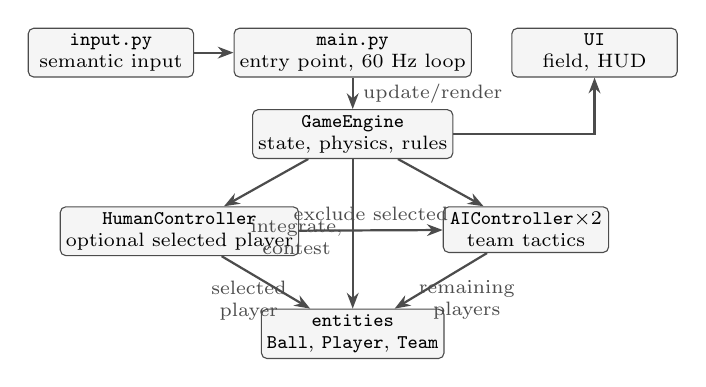
\begin{tikzpicture}[node distance=4mm and 6mm]
  \node[block] (main) {\code{main.py}\\entry point, 60 Hz loop};
  \node[block, below=of main] (engine) {\code{GameEngine}\\state, physics, rules};
  \node[block, left=5mm of main] (input) {\code{input.py}\\semantic input};
  \node[block, below=6mm of engine, xshift=-22mm] (human) {\code{HumanController}\\optional selected player};
  \node[block, below=6mm of engine, xshift=22mm] (ai) {\code{AIController}$\times2$\\team tactics};
  \node[block, below=19mm of engine] (ent) {\code{entities}\\\code{Ball}, \code{Player}, \code{Team}};
  \node[block, right=5mm of main] (ui) {\code{UI}\\field, HUD};
  \draw[arrow] (main) -- node[lbl,right]{update/render} (engine);
  \draw[arrow] (input) -- (main);
  \draw[arrow] (engine) -- (human);
  \draw[arrow] (engine) -- (ai);
  \draw[arrow] (human) -- node[lbl,left,pos=0.85]{selected\\player} (ent);
  \draw[arrow] (human) -- node[lbl,above]{exclude selected} (ai);
  \draw[arrow] (ai) -- node[lbl,right,pos=0.85]{remaining\\players} (ent);
  \draw[arrow] (engine) -- node[lbl,left,pos=0.52]{integrate,\\contest} (ent);
  \draw[arrow] (engine.east) -| (ui.south);
\end{tikzpicture}
\caption{Runtime architecture. The engine owns world state and rules. In
all-AI mode it updates both team controllers directly; in mixed-control mode
semantic input drives one selected player through \code{HumanController},
which delegates all remaining teammates to the same tactical AI.}
\label{fig:architecture}
\end{figure}

The runtime is organised as seven cooperating modules
(\cref{fig:architecture}). The
\code{GameEngine} owns the world state --- field geometry, ball, two teams,
score, clock, controller routing and restart bookkeeping --- and enforces all
rules. Two symmetric \code{AIController} instances, one per team, observe the
full state (perception is perfect and global; there is no sensor noise). In
all-AI mode they issue every steering and kick command. In mixed-control mode
the designated side is routed through \code{HumanController}: it excludes the
selected player from that side's AI update, then applies semantic input to
that player only. Entities integrate their own dynamics. The renderer draws
the pitch, players, possession halo, goalkeeper rings, stamina bars, the
human-selection chevron and a HUD with score, clock, possession shares, shot
counts and a conditional controls legend; it is not needed for simulation
and is bypassed in headless experiments (\cref{sec:setup}).

The field is an $F_W \times F_H = 700 \times 500\px$ rectangle with margins
inside an $800\times600$ window; each goal mouth spans the central 40\% of
the goal line, $[0.3F_H,\,0.7F_H]$. Each team fields six agents in a
2--2--1+GK formation (\cref{tab:formation}); Team~2's slots mirror Team~1's
horizontally ($f_x \mapsto 1-f_x$).

\begin{table}[t]
\centering\small
\caption{Formation slots as fractions $(f_x,f_y)$ of the field, for the
team attacking rightward. The home position is
$(x_0 + f_x F_W,\; y_0 + f_y F_H)$.}
\label{tab:formation}
\begin{tabular}{@{}llcc@{}}
\toprule
Slot & Role & $f_x$ & $f_y$ \\
\midrule
P1 & defender    & 0.18 & 0.35 \\
P2 & defender    & 0.18 & 0.65 \\
P3 & midfielder  & 0.40 & 0.30 \\
P4 & midfielder  & 0.40 & 0.70 \\
P5 & striker     & 0.62 & 0.50 \\
P6 & goalkeeper  & 0.03 & 0.50 \\
\bottomrule
\end{tabular}
\end{table}

\subsection{Control Modes and Human Interface}\label{sec:human}

\code{GameEngine(human\_team=None)} is the reproducible all-AI mode used by
the headless monitor and every experiment in \cref{sec:setup}. The interactive
entry point instead constructs \code{GameEngine(human\_team="team1")}: Team~1
is mixed human/AI and Team~2 remains autonomous. Raw pygame events are
translated by \code{input.py} into an \code{InputFrame} containing a
normalised eight-direction movement vector, one-frame action edges and held
modifiers. Controllers therefore consume semantic actions rather than key
codes, keeping input rebindable and unit-testable.

\begin{table}[t]
\centering\small
\caption{Default interactive controls. Movement and sprint are continuous;
pass, shoot and player switch are edge-triggered.}
\label{tab:controls}
\begin{tabular}{@{}ll@{}}
\toprule
Intent & Default binding \\
\midrule
Move & W/A/S/D or arrow keys \\
Sprint & either Shift key (held) \\
Pass & J \\
Shoot & K \\
Switch defender & Tab \\
Pause / reset / quit & Space / R / Escape \\
\bottomrule
\end{tabular}
\end{table}

The human controls exactly one player. In possession, selection follows the
carrier, so control transfers naturally to a receiver when a pass is
collected; this includes the goalkeeper while it holds the ball. Out of
possession, the nearest outfield player to the ball is selected automatically
and repeated switch actions cycle through the distance-ordered outfield list.
The goalkeeper is excluded from defensive auto-selection and switching, not
from on-ball control.
The selected player steers toward a point $20\px$ along the input vector at
normal maximum speed, or at $1.3$ times that speed while sprint is held.
Because this is an ordinary movement command, the existing stamina-dependent
speed factor and high-speed drain remain in force.

Human shots reuse the AI's blocker-aware corner-selection procedure. Human
passes use a direct-control heuristic instead: choose the nearest non-keeper
teammate whose direction has dot product at least $0.3$ with the current aim,
falling back to the nearest teammate when the cone is empty. Unlike AI
passing, this convenience heuristic does not veto blocked lanes or offside
positions; offside remains a pass-selection policy rather than an
engine-level whistle. Passes and shots still call the same entity methods,
pay the same stamina costs and obey the same action cooldowns as AI actions.

The AI continues to position every unselected teammate. Before its update the
human controller sets \code{AIController.controlled\_player}; all tactical
roles, including presser, support runner, carrier and goalkeeper, exclude that
player from AI commands while retaining it in the roster for possession and
team-state calculations. Thus a selected goalkeeper is driven by human input
until it releases the ball, rather than by the three-mode keeper policy of
\cref{sec:keeper}. This exclusion boundary prevents double commands.
Neither the input layer nor the human controller can assign possession:
human and AI players enter the same central contest of
\cref{sec:contest}, use the same restart entitlement, and are subject to the
same tackle, foul, cooldown and stamina rules.

\subsection{Discrete-Time Integration and Friction}\label{sec:physics}

The world advances with a variable timestep $\Delta t$ (fixed at
$0.016$~s in experiments by the harness's integer-millisecond clock). All
entities are point masses with position
$\mathbf{x}$ and velocity $\mathbf{v}$ updated by a drift-then-decay scheme:
\begin{equation}\label{eq:integrate}
\mathbf{x}_{t+\Delta t} = \mathbf{x}_t + \mathbf{v}_t\,\Delta t,
\qquad
\mathbf{v}_{t+\Delta t} = \mathbf{v}_t\,\mu^{\Delta t},
\end{equation}
where $\mu \in (0,1)$ is the fraction of velocity retained after one second
of free movement: $\mu_e = 0.046$ for players (calibrated to reproduce the
legacy per-frame factor $0.95^{60}\!\approx\!0.046$ at 60~Hz) and
$\mu_b = 0.05$ for the rolling ball. The exponential makes velocity
attenuation over a fixed elapsed time independent of frame rate. Position is
advanced before the decay, however, so the sampled trajectory retains the
ordinary timestep error of the discrete drift and is not exactly invariant
across frame rates. In the continuous-time limit the decay corresponds to the
linear drag law
$\dot{\mathbf v} = -\lambda \mathbf v$ with rate
\begin{equation}\label{eq:lambda}
\lambda \;=\; -\ln \mu_b \;\approx\; 3.00\ \text{s}^{-1},
\end{equation}
so a ball kicked at speed $v_0$ travels a total distance
\begin{equation}\label{eq:reach}
d_{\infty} \;=\; \int_0^{\infty} v_0 e^{-\lambda t}\,dt \;=\; \frac{v_0}{\lambda},
\end{equation}
a closed form the kick model inverts to power kicks by intended range
(\cref{sec:kick}). Ball speed is capped at $V_{\max}=900\pxs$ before each
integration step, preventing tunnelling through players or walls, and a
wall bounce (used only for a virgin ball that has never been touched, see
\cref{sec:restarts}) reflects the normal velocity component with
restitution $e = 0.8$.

\subsection{Kick Model}\label{sec:kick}

Kicks are instantaneous velocity assignments. A kick toward direction
$\hat{\mathbf u}$ with power $P$ and current stamina factor
$\phi \in [\phi_{\min},1]$ (see \cref{sec:stamina}) sets
\begin{equation}\label{eq:kick}
\mathbf v_{\text{ball}} \;=\; P\,\phi\;\hat{\mathbf u},
\end{equation}
releases possession, and starts an in-flight window of
$\tau_{\text{loose}} = 0.3$~s during which no player may control the ball
--- without it, the kicker would recapture its own shot on the next frame.
Each kick also starts the kicker's action cooldown
$\tau_{\text{act}} = 0.5$~s.

Powers are sized by inverting \cref{eq:reach}. A pass over distance $d$
should die near the receiver's feet, so
\begin{equation}\label{eq:passpower}
P_{\text{pass}}(d) \;=\;
\min\!\bigl(\max(d\,\lambda\,\gamma_p,\; P_{\min}),\; V_{\max}\bigr),
\end{equation}
with margin $\gamma_p = 1.1$ (the ball arrives with residual pace) and
floor $P_{\min}=200\pxs$ so tap passes still zip. A shot over distance $d$
must \emph{arrive} fast rather than die on the line, hence a larger margin
$\gamma_s = 1.25$ and a floor at the player's base shot power
$P_0 = 500\pxs$:
\begin{equation}\label{eq:shotpower}
P_{\text{shot}}(d) \;=\;
\max\!\bigl(P_0,\; \min(d\,\lambda\,\gamma_s,\; P_{\max})\bigr),
\quad P_{\max}=900\pxs .
\end{equation}

While possessed, the ball is \emph{carried}: each frame it is glued at
offset $(r_p + r_b)$ ahead of the carrier along its facing direction and
inherits the carrier's velocity, so dribbling moves the ball and a
subsequent kick starts from a sensible motion state. Passing first turns
the carrier toward the receiver (updating the facing direction and
re-gluing the ball on that side) so back-passes are kicked from the correct
side of the body.

\subsection{Stamina Model}\label{sec:stamina}

Each player carries a stamina reservoir $s \in [0, S]$, $S=100$, coupling
effort to both speed and kick power. With speed ratio
$\rho = \lVert\mathbf v\rVert / v_{\max}$, stamina evolves as
\begin{equation}\label{eq:stamina}
\dot s \;=\;
\begin{cases}
-\,c_{\text{sprint}}\;\rho, & \rho > \rho_{\text{sprint}} \\
+\,c_{\text{rec}}, & \rho < \rho_{\text{rec}} \\
0, & \text{otherwise,}
\end{cases}
\end{equation}
with $\rho_{\text{sprint}}=0.75$, $\rho_{\text{rec}}=0.5$,
$c_{\text{sprint}}=2.5\,\text{s}^{-1}$ and $c_{\text{rec}}=5\,\text{s}^{-1}$;
each shot additionally costs 10 units and each pass 5. Fatigue acts through
two floored linear factors, a speed factor $\psi$ and a power factor
$\phi$:
\begin{equation}\label{eq:factors}
\psi(s) = \psi_{\min} + (1-\psi_{\min})\frac{s}{S},
\qquad
\phi(s) = \phi_{\min} + (1-\phi_{\min})\frac{s}{S},
\end{equation}
with $\psi_{\min}=0.85$ and $\phi_{\min}=0.8$: an exhausted player still
moves at 85\% pace and kicks at 80\% power. The system is deliberately
self-stabilising --- a tired player slows down, drops below
$\rho_{\text{sprint}}$, and stops draining --- so stamina adds texture
without collapsing match tempo, a failure mode observed in early versions.

\subsection{Movement Model}\label{sec:movement}

Agents do not teleport onto command velocities. A movement command toward
target $\mathbf T$ at requested speed $v$ produces a desired velocity
$\mathbf v^{*} = \psi(s)\,v\,\widehat{(\mathbf T - \mathbf x)}$ and blends
the current velocity toward it:
\begin{equation}\label{eq:blend}
\mathbf v \leftarrow \mathbf v + \bigl(\mathbf v^{*} - \mathbf v\bigr)\,\alpha(\Delta t),
\qquad
\alpha(\Delta t) = 1 - (1-\beta)^{\Delta t\, f_0},
\end{equation}
with per-frame blend $\beta = 0.25$ at reference rate $f_0 = 60$~Hz. Since
the AI re-issues commands every frame, repeated application converges
geometrically to $\mathbf v^{*}$; starts, stops and turns therefore take a
few frames, giving players momentum, and \cref{eq:blend} is again
frame-rate independent by construction. The same exponential-rescaling
idea converts tuned per-frame decision probabilities to arbitrary
timesteps:
\begin{equation}\label{eq:prob}
p(\Delta t) \;=\; 1 - (1 - p_{60})^{\Delta t\, f_0},
\end{equation}
used by every stochastic decision in \cref{sec:behaviour}.

\begin{table}[t]
\centering\small
\begin{threeparttable}
\caption{Principal physics and rules parameters (repository defaults).}
\label{tab:physparams}
\begin{tabular}{@{}llS[table-format=3.2]@{}}
\toprule
Symbol & Meaning & {Value} \\
\midrule
$\mu_b$ & ball velocity retained per second & 0.05 \\
$\mu_e$ & player velocity retained per second & 0.046 \\
$V_{\max}$ & ball speed cap (\pxs) & 900 \\
$e$ & wall restitution & 0.8 \\
$\gamma_p,\ \gamma_s$ & pass / shot power margin & {1.1 / 1.25} \\
$P_{\min},\ P_0$ & pass floor / base shot power (\pxs) & {200 / 500} \\
$\tau_{\text{loose}}$ & in-flight (uncontrollable) window (s) & 0.30 \\
$\tau_{\text{act}}$ & action cooldown after a kick (s) & 0.50 \\
$p_{\text{tackle}}$ & tackle success per frame\tnote{a} & 0.05 \\
$p_{\text{foul}}$ & foul given a won tackle & 0.15 \\
$\tau_{\text{foul}}$ & fouler booking cooldown (s) & 1.5 \\
$\beta$ & movement blend per 60 Hz frame & 0.25 \\
$\rho_{\text{sprint}},\ \rho_{\text{rec}}$ & sprint / recovery thresholds & {0.75 / 0.5} \\
$\psi_{\min},\ \phi_{\min}$ & speed / power floors & {0.85 / 0.8} \\
\bottomrule
\end{tabular}
\begin{tablenotes}\footnotesize
\item[a] Swept in \cref{sec:results}; per-frame at 60 Hz.
\end{tablenotes}
\end{threeparttable}
\end{table}

% =============================================================================
\section{Rules and Possession Model}\label{sec:rules}

\subsection{The Engine Step}\label{sec:step}

\cref{alg:step} and \cref{fig:steploop} give the per-frame pipeline. Its
ordering embeds three design decisions. First, a pending kickoff pass is
executed \emph{before} the team controllers act, so restarts cannot be pre-empted.
Second, possession is resolved centrally \emph{after} both AI controllers
or the optional human controller and all integrations have run: an earlier
design let each team controller grab the ball for its own players, which
handed possession to whichever controller happened to run last every frame
(the baseline report measured 0.0\% possession for Team~1 as a result).
Third, ball--boundary handling runs last, on the final ball position of the
frame.

\begin{algorithm}[t]
\caption{Engine step (one frame).}
\label{alg:step}
\begin{algorithmic}[1]
\State $\Delta t \gets$ elapsed time; advance match clock
\If{kickoff pending} \State attempt kickoff pass (\cref{sec:restarts})
\EndIf
\State \textsc{UpdateControllers}$(\Delta t)$ \Comment{AI or mixed human/AI by team}
\State integrate ball (\cref{eq:integrate}, speed cap)
\ForAll{players $p$} integrate $p$; clamp $\mathbf x_p$ to field
\EndFor
\State \textsc{ResolvePossession()} \Comment{\cref{alg:possession}}
\State accrue possession time for the holder's team
\State \textsc{SeparatePlayers()} \Comment{\cref{sec:separation}}
\If{ball possessed} glue ball to carrier (\cref{sec:kick})
\EndIf
\State \textsc{HandleBallBoundaries()} \Comment{goals, restarts; \cref{sec:restarts}}
\end{algorithmic}
\end{algorithm}

\begin{figure}[t]
\centering
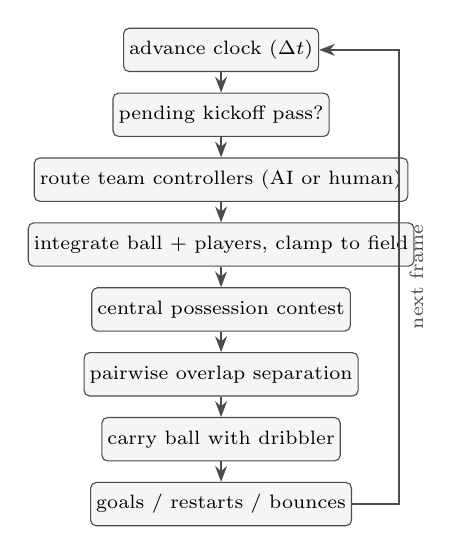
\begin{tikzpicture}[node distance=2.6mm]
  \node[block] (dt) {advance clock ($\Delta t$)};
  \node[block, below=of dt] (ko) {pending kickoff pass?};
  \node[block, below=of ko] (ctrl) {route team controllers (AI or human)};
  \node[block, below=of ctrl] (integ) {integrate ball + players, clamp to field};
  \node[block, below=of integ] (poss) {central possession contest};
  \node[block, below=of poss] (sep) {pairwise overlap separation};
  \node[block, below=of sep] (carry) {carry ball with dribbler};
  \node[block, below=of carry] (bound) {goals / restarts / bounces};
  \draw[arrow] (dt) -- (ko);
  \draw[arrow] (ko) -- (ctrl);
  \draw[arrow] (ctrl) -- (integ);
  \draw[arrow] (integ) -- (poss);
  \draw[arrow] (poss) -- (sep);
  \draw[arrow] (sep) -- (carry);
  \draw[arrow] (carry) -- (bound);
  \draw[arrow] (bound.east) -- ++(6mm,0) |- node[lbl, right, pos=0.25, rotate=90, anchor=north]{next frame} (dt.east);
\end{tikzpicture}
\caption{Per-frame control flow of the engine step (\cref{alg:step}).}
\label{fig:steploop}
\end{figure}

\subsection{Order-Independent Possession Contest}\label{sec:contest}

Possession is a discrete state: at most one player holds the ball.
\cref{alg:possession} resolves it once per frame. A player is
\emph{eligible} to take the ball if it is within control range
($\lVert\mathbf x_p - \mathbf x_b\rVert < r_p + r_b + 5\px$), off action
cooldown, and --- during a restart --- belongs to the entitled team. A free
ball goes to the nearest eligible player. A held ball can only change hands
through a probabilistic tackle: with per-frame probability
$p_{\text{tackle}} = 0.05$ the nearest contesting opponent wins it, except
that with conditional probability $p_{\text{foul}} = 0.15$ the challenge is
whistled as a foul --- the holder retains the ball (a simplified free kick)
and the fouler is booked with a $\tau_{\text{foul}}=1.5$~s cooldown that
bars an immediate re-challenge. Teammates never steal from each other, and
a kicker on cooldown cannot instantly reclaim its own kick.

\begin{algorithm}[t]
\caption{\textsc{ResolvePossession} --- fair per-frame contest.}
\label{alg:possession}
\begin{algorithmic}[1]
\If{$\text{ball.looseTimer} > 0$} \Return \Comment{in flight: nobody controls}
\EndIf
\State $h \gets$ ball.holder
\If{$h \neq \varnothing$ \textbf{and} $h$ out of control range} $h \gets \varnothing$
\EndIf
\State $E \gets \{p \neq h : p \text{ in range} \wedge p \text{ off cooldown} \wedge{}$
\Statex \hspace{\algorithmicindent}\hphantom{$E \gets \{$}$(\text{no restart} \vee p \in \text{entitled team})\}$
\If{$h = \varnothing$}
  \If{$E \neq \emptyset$} holder $\gets \arg\min_{p \in E} \lVert\mathbf x_p - \mathbf x_b\rVert$; clear restart
  \EndIf
  \State \Return
\EndIf
\State $O \gets \{p \in E : \text{team}(p) \neq \text{team}(h)\}$
\If{$O \neq \emptyset$ \textbf{and} $\mathrm{U}(0,1) < p_{\text{tackle}}$}
  \State $q \gets \arg\min_{p \in O} \lVert\mathbf x_p - \mathbf x_b\rVert$
  \If{$\mathrm{U}(0,1) < p_{\text{foul}}$} book $q$ for $\tau_{\text{foul}}$ \Comment{holder keeps ball}
  \Else\ holder $\gets q$
  \EndIf
\EndIf
\end{algorithmic}
\end{algorithm}

\subsection{Restarts, Goals and Boundaries}\label{sec:restarts}

A goal is scored when the ball's centre crosses a goal line within the goal
mouth; the conceding team then restarts with a kickoff. At kickoff, every
player is placed at its formation home clamped into its own half (margin
$20\px$ from the halfway line; the non-kicking team additionally respects a
$60\px$ margin, keeping it outside the centre circle), the most advanced
outfield player of the kicking team stands on the centre spot with the
ball, and passes to one of its two nearest outfield teammates chosen
uniformly at random --- randomising the receiver keeps restarts from
looking scripted. \cref{fig:kickoff} shows the opening lineup.

Any other exit of the ball awards a \emph{restart} against the team that
last touched it: a throw-in at the sideline crossing point, a corner at the
nearest corner (defender touched last) or a goal kick placed $40\px$ in
front of the goal (attacker touched last). A restart is a dead ball --- the
engine zeroes the ball velocity at the restart point and marks the entitled
team; only that team's players may take possession
(\cref{alg:possession}), while the AI's ordinary chase behaviour sends its
nearest player to collect. A ball carried over a line by a dribbler counts
as conducted out by the carrier's team, closing a loophole in which
carriers could grind along the boundary indefinitely. Only a ball that has
never been touched (no attributable last toucher) falls back to a physical
wall bounce with restitution $e$.

Offside is simplified to a positional predicate used by pass selection
(receivers in offside position are simply never targeted). A player $p$ of
the team attacking in direction $\sigma \in \{+1,-1\}$ is offside iff
\begin{equation}\label{eq:offside}
\underbrace{(x_p - x_c)\,\sigma > 0}_{\text{in opponent half}}
\;\wedge\;
\underbrace{(x_p - x_b)\,\sigma > 0}_{\text{ahead of the ball}}
\;\wedge\;
\underbrace{(x_p - x_{(2)})\,\sigma > 0}_{\text{past 2nd-last opponent}},
\end{equation}
where $x_c$ is the halfway line, $x_b$ the ball and $x_{(2)}$ the
second-last opponent's $x$ (the last is usually the goalkeeper, so
$x_{(2)}$ marks the effective defensive line, as in the real law).

\subsection{Collision Resolution}\label{sec:separation}

Players are rigid discs of radius $r_p = 10\px$. After integration, every
overlapping pair $(a,b)$ is separated along the line of centres: each
player moves half the overlap outward, positions are re-clamped to the
field, and any overlap remaining because a clamp absorbed part of the push
is redistributed to whichever player can still move. This single-pass
positional projection removes the pathological stacking of the prototype
(98.4\% of frames crossed the old severe-overlap threshold of $15\px$).
Post-fix measurements in \cref{sec:results} show no severe overlaps and
$1.6\%$ geometric overlap at the stricter $20\px$ disc-contact threshold.

% =============================================================================
\section{Team Behaviour Model}\label{sec:behaviour}

\subsection{Team State Machine and Role Assignment}\label{sec:states}

Each controller classifies every frame into one of three team states
(\cref{fig:states}): \textsc{attack} if a teammate holds the ball,
\textsc{defense} if an opponent does, and, for a free ball, \textsc{possession}
(chase) if the team's nearest outfield player is closer to the ball than
the opponents' nearest, else \textsc{defense}. Exactly one player --- the
\emph{active} player --- presses or carries the ball; in \textsc{attack} the
nearest non-defender teammate becomes the \emph{support} runner
(\cref{sec:support}); everyone else holds tactical shape. The goalkeeper is
exempt from all outfield duties and runs a dedicated policy
(\cref{sec:keeper}) that overrides any formation movement assigned to it.

\begin{figure}[t]
\centering
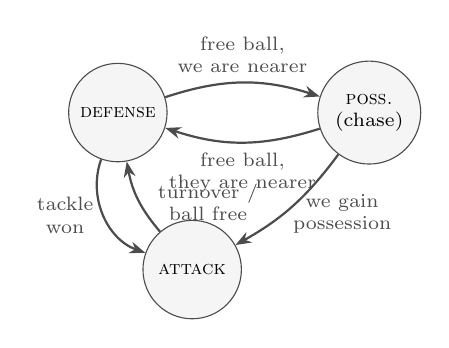
\begin{tikzpicture}[node distance=1.5cm and 1.9cm]
  \node[state] (def) {\textsc{defense}};
  \node[state, right=of def] (pos) {\textsc{poss.}\\(chase)};
  \node[state, below right=1.1cm and 0.05cm of def] (att) {\textsc{attack}};
  \draw[arrow] (def) edge[bend left=18] node[lbl, above]{free ball,\\we are nearer} (pos);
  \draw[arrow] (pos) edge[bend left=18] node[lbl, below]{free ball,\\they are nearer} (def);
  \draw[arrow] (pos) edge[bend left=12] node[lbl, right, pos=0.6]{we gain\\possession} (att);
  \draw[arrow] (att) edge[bend left=15] node[lbl, right, pos=0.45, xshift=1mm]{turnover /\\ball free} (def);
  \draw[arrow] (def) edge[bend right=45] node[lbl, left, pos=0.5]{tackle\\won} (att);
\end{tikzpicture}
\caption{Per-frame team state classification. Both controllers evaluate the
same shared state symmetrically.}
\label{fig:states}
\end{figure}

\subsection{Elastic Formation Shape}\label{sec:formation}

Off-ball players in neutral situations hold an \emph{elastic formation}: the
whole block translates toward the ball while preserving relative role
geometry, instead of collapsing onto the ball. With ball position
$\mathbf b$, field centre $\mathbf c$, home position $\mathbf h_i$ and
attack direction $\sigma$, player $i$'s shape target is
\begin{equation}\label{eq:formation}
\mathbf T_i \;=\; \Pi_{\mathcal F}\!\Bigl[\,\mathbf h_i
   + \kappa_{\text{slide}}\,(\mathbf b - \mathbf c)
   + \delta\,\sigma\,\hat{\mathbf e}_x \Bigr],
\end{equation}
\begin{equation}\label{eq:pushdrop}
\delta =
\begin{cases}
+130\px & \text{in \textsc{attack}} \\
-60\px & \text{in \textsc{defense}} \\
\hphantom{+}0 & \text{otherwise,}
\end{cases}
\end{equation}
where $\kappa_{\text{slide}} = 0.5$ is the slide gain (swept in
\cref{sec:results}) and $\Pi_{\mathcal F}$ clamps the target at least
$35\px$ inside the field so shape survives near boundaries. The
asymmetric push/drop $\delta$ gives attacking depth and defensive
compactness.

\subsection{Defensive Organisation}\label{sec:defense}

Out of possession the team defends in three coordinated mechanisms,
selected by threat level (distance from the ball to the defended goal).

\paragraph{Two-bank block (low threat).} When the ball is farther than
$300\px$ from the goal, defenders and midfielders form two flat banks
perpendicular to the pitch axis (\cref{fig:defblock}). The bank depths and
the gap between them scale linearly with the normalised ball distance
$t = \min\!\bigl(1, d_x(\mathbf b, \text{goal})/F_W\bigr)$:
\begin{align}\label{eq:block}
D(t) &= D_{\min} + (D_{\max}-D_{\min})\,t, \\
G(t) &= G_{\min} + (G_{\max}-G_{\min})\,t, \notag
\end{align}
with $D \in [80, 240]\px$ and $G \in [60,120]\px$: the block retreats and
compresses as the attack advances, and steps up and stretches as it
recedes. Within a bank, teammates are spaced $100\px$ apart, centred on a
lateral anchor that follows the ball with gain $0.6$, and slots are
assigned by home-$y$ order so teammates never swap sides.

\paragraph{Goal-side man-marking (high threat).} When the ball comes within
$300\px$ of the goal, off-ball defenders switch to man-marking. Markers and
targets (opponents within $320\px$ of the goal, except their carrier) are
paired by greedy nearest-first matching --- sort all marker--target pairs
by distance and take them in order, one marker per target --- and each
marker stands at the goal-side point
\begin{equation}\label{eq:mark}
\mathbf m \;=\; \mathbf o + M\,\frac{\mathbf g - \mathbf o}{\lVert \mathbf g - \mathbf o \rVert},
\qquad M = 22\px,
\end{equation}
between its man $\mathbf o$ and the goal centre $\mathbf g$
(\cref{fig:marking}). A defender left goal-side of the ball with no man to
mark converges on the carrier instead of loitering on its own goal line as
an extra keeper.

\paragraph{Rest defence (own possession).} While the team attacks, its two
defenders do not join the push: they hold a flat cover line goal-side of
the ball (\cref{fig:restdef}) at depth
\begin{equation}\label{eq:rest}
D_{\text{rest}} \;=\;
\operatorname{clip}\bigl(d_x(\mathbf b,\text{goal}) - 130,\; 130,\; 330\bigr)\px,
\end{equation}
trailing the ball by $130\px$ but never collapsing onto the keeper nor
crossing the halfway area, with a gentle lateral follow (gain $0.4$). A
turnover therefore never yields an uncontested counter-attack.

\subsection{Attacking Play: the Carrier Policy}\label{sec:attack}

The ball carrier follows the prioritised stochastic policy of
\cref{alg:carrier} and \cref{fig:carrierflow}: shoot when close with a
good angle; occasionally strike from long range; under pressure,
probabilistically offload; in build-up, pass only when it clearly improves
the team's position; otherwise dribble.

\begin{algorithm}[t]
\caption{Carrier decision policy (one frame, carrier $k$).}
\label{alg:carrier}
\begin{algorithmic}[1]
\State $d \gets \lVert \mathbf x_k - \mathbf g_{\text{opp}} \rVert$;\quad
$\theta \gets$ shot angle (\cref{eq:angle});\quad acted $\gets$ \textbf{false}
\State pressured $\gets \exists$ opponent within $30\px$ of $k$
\If{$k$ off cooldown}
 \If{$d < R_{\text{shot}}$ \textbf{and} $\theta \ge \theta_{\min}$}
   \State shoot at corner target (\cref{eq:aim}); acted $\gets$ \textbf{true}
 \ElsIf{$d < R_{\text{long}}$ \textbf{and} $\theta \ge \theta_{\min}$ \textbf{and} $\mathrm{U} < p(\Delta t; p_{\text{long}})$}
   \State long-range shot (\cref{eq:shotpower}); acted $\gets$ \textbf{true}
 \ElsIf{pressured \textbf{and} $\mathrm{U} < p(\Delta t; p_{\text{off}})$}
   \State $r \gets \textsc{BestPassTarget}(k, \text{backward allowed})$
   \If{$r \neq \varnothing$} pass to $r$; acted $\gets$ \textbf{true}
   \EndIf
 \ElsIf{\textbf{not} pressured}
   \State $r \gets \textsc{BestPassTarget}(k)$ \Comment{forward only}
   \If{$r \neq \varnothing$ \textbf{and} $\omega(r) > \omega(k) + 5$} pass to $r$; acted $\gets$ \textbf{true}
   \EndIf
 \EndIf
\EndIf
\If{\textbf{not} acted}
  \State dribble $20\px$ goalward; steer to widen a tight angle and
         around a presser; clamp target $\ge 25\px$ inside the field
\EndIf
\end{algorithmic}
\end{algorithm}

\begin{figure}[t]
\centering
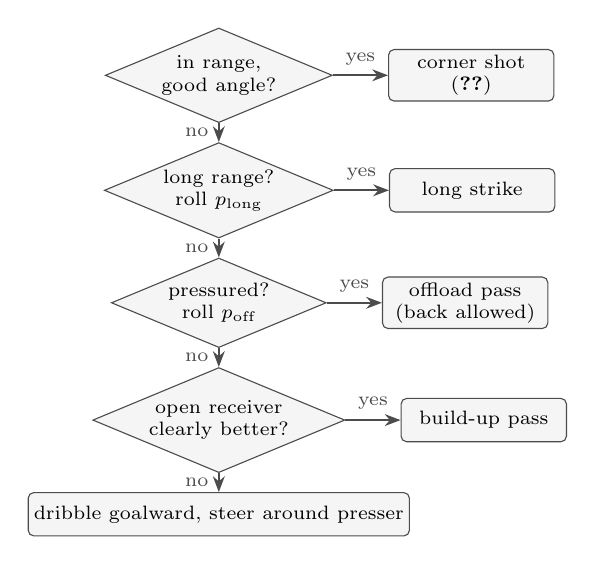
\begin{tikzpicture}[node distance=2.4mm]
  \node[decision] (shot) {in range,\\good angle?};
  \node[block, right=7mm of shot] (doshot) {corner shot\\(\cref{eq:aim})};
  \node[decision, below=of shot] (long) {long range?\\roll $p_{\text{long}}$};
  \node[block, right=7mm of long] (dolong) {long strike};
  \node[decision, below=of long] (press) {pressured?\\roll $p_{\text{off}}$};
  \node[block, right=7mm of press] (dooff) {offload pass\\(back allowed)};
  \node[decision, below=of press] (build) {open receiver\\clearly better?};
  \node[block, right=7mm of build] (dopass) {build-up pass};
  \node[block, below=of build] (drib) {dribble goalward, steer around presser};
  \draw[arrow] (shot) -- node[lbl,above]{yes} (doshot);
  \draw[arrow] (shot) -- node[lbl,left]{no} (long);
  \draw[arrow] (long) -- node[lbl,above]{yes} (dolong);
  \draw[arrow] (long) -- node[lbl,left]{no} (press);
  \draw[arrow] (press) -- node[lbl,above]{yes} (dooff);
  \draw[arrow] (press) -- node[lbl,left]{no} (build);
  \draw[arrow] (build) -- node[lbl,above]{yes} (dopass);
  \draw[arrow] (build) -- node[lbl,left]{no} (drib);
\end{tikzpicture}
\caption{Carrier decision flow (\cref{alg:carrier}). Every stochastic
gate uses the frame-rate--corrected probability of \cref{eq:prob}; any
branch that fails to fire falls through to dribbling.}
\label{fig:carrierflow}
\end{figure}

\paragraph{Decision passing.} Pass selection
(\cref{alg:pass}) filters teammates through five vetoes --- range,
direction, openness (long balls only), offside (\cref{eq:offside}) and
lane occlusion --- then maximises a composite score. The \emph{openness}
of a player is its distance to the nearest opponent,
\begin{equation}\label{eq:openness}
\omega(p) \;=\; \min_{o \in \text{opponents}} \lVert \mathbf x_p - \mathbf x_o \rVert ,
\end{equation}
and a candidate receiver $r$ is scored by
\begin{equation}\label{eq:passscore}
J(r) \;=\; \omega(r) \;-\; \tfrac{1}{2}\,\bigl| x_{\text{goal}} - x_r \bigr|,
\end{equation}
trading off freedom from marking against progress toward the goal. Short
passes are allowed up to $130\px$; \emph{forward} receivers up to $260\px$
qualify for a driven long ball, but only when clearly open,
$\omega(r) \ge 60\px$, relaxed to $30\px$ if the receiver is already in
shooting range (a killer ball into the box justifies more risk). The lane
veto (\cref{fig:lane}) rejects receivers whose straight passing corridor
is occluded: for each opponent $\mathbf o$, project onto the pass segment
$\mathbf p \to \mathbf q$,
\begin{equation}\label{eq:lane}
t^{\ast} = \frac{(\mathbf o - \mathbf p)\cdot(\mathbf q - \mathbf p)}
               {\lVert \mathbf q - \mathbf p \rVert^{2}},
\qquad
d^{\ast} = \bigl\lVert \mathbf o - \bigl(\mathbf p + t^{\ast}(\mathbf q - \mathbf p)\bigr) \bigr\rVert,
\end{equation}
and the lane is blocked iff $t^{\ast} \in [0.15, 1]$ and $d^{\ast} < 25\px$.
Opponents projecting onto the first 15\% of the segment are deliberately
ignored --- an opponent beside the carrier is the \emph{pressure}
situation, handled by the offload gate, not an occluded lane. In build-up
(no pressure) a pass additionally requires
$\omega(r) > \omega(k) + 5\px$, i.e.\ it must strictly improve the team's
position rather than cycle the ball; under pressure a backward outlet is
permitted.

\begin{figure}[t]
\centering
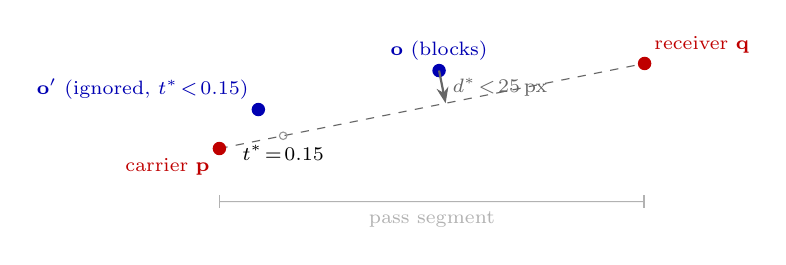
\begin{tikzpicture}[scale=0.9]
  \coordinate (P) at (0,0);
  \coordinate (Q) at (6,1.2);
  \coordinate (O1) at (3.1,1.1);
  \coordinate (O2) at (0.55,0.55);
  \draw[dashed, black!60] (P) -- (Q);
  \fill[red!75!black] (P) circle (2.7pt) node[below left, font=\scriptsize]{carrier $\mathbf p$};
  \fill[red!75!black] (Q) circle (2.7pt) node[above right, font=\scriptsize]{receiver $\mathbf q$};
  \fill[blue!70!black] (O1) circle (2.7pt) node[above, font=\scriptsize]{$\mathbf o$ (blocks)};
  \fill[blue!70!black] (O2) circle (2.7pt) node[above left, font=\scriptsize]{$\mathbf o'$ (ignored, $t^{\ast}\!<\!0.15$)};
  % projection of O1
  \coordinate (H) at ($(P)!(O1)!(Q)$);
  \draw[arrow, black!60] (O1) -- node[lbl, right]{$d^{\ast}\!<\!25\px$} (H);
  \draw[black!40] ($(P)!0.15!(Q)$) circle (1.5pt);
  \node[font=\scriptsize, below] at ($(P)!0.15!(Q)$) {$t^{\ast}\!=\!0.15$};
  \draw[black!30, |-|] ($(P)+(0,-0.75)$) -- node[lbl, below]{pass segment} ($(Q)+(0,-1.95)$);
\end{tikzpicture}
\caption{Lane occlusion test of \cref{eq:lane}. Opponent $\mathbf o$
projects inside $[0.15,1]$ within $25\px$ of the corridor and vetoes the
pass; $\mathbf o'$ is adjacent to the carrier and is handled by the
pressure gate instead.}
\label{fig:lane}
\end{figure}

\begin{algorithm}[t]
\caption{\textsc{BestPassTarget}$(k,\ \text{allowBackward})$.}
\label{alg:pass}
\begin{algorithmic}[1]
\Function{Candidates}{$k$, forward}
  \State $C \gets \emptyset$
  \ForAll{teammates $p \neq k$}
    \State $d \gets \lVert \mathbf x_p - \mathbf x_k \rVert$;\quad
           $R \gets$ forward ? $260$ : $130$
    \If{$d > R$ \textbf{or} direction$(p)\neq$ forward} \textbf{continue} \EndIf
    \If{$d > 130$ \textbf{and} $\omega(p) < $ (in shot range ? $30$ : $60$)} \textbf{continue} \EndIf
    \If{offside$(p)$ (\cref{eq:offside}) \textbf{or} lane blocked (\cref{eq:lane})} \textbf{continue} \EndIf
    \State $C \gets C \cup \{p\}$
  \EndFor
  \State \Return $C$
\EndFunction
\State $C \gets \Call{Candidates}{k, \text{forward}}$
\If{$C = \emptyset$ \textbf{and} allowBackward} $C \gets \Call{Candidates}{k, \text{backward}}$
\EndIf
\State \Return $\arg\max_{r \in C} J(r)$ (\cref{eq:passscore}), or $\varnothing$
\end{algorithmic}
\end{algorithm}

\paragraph{Shooting.} A shot is gated by range and by the \emph{shot
angle}: the angular width of the goal mouth as seen from the shooter,
\begin{equation}\label{eq:angle}
\theta(\mathbf x) \;=\;
\Bigl| \operatorname{atan2}(y_{\text{top}} - y,\; x_g - x)
     - \operatorname{atan2}(y_{\text{bot}} - y,\; x_g - x) \Bigr| ,
\end{equation}
The implementation uses this raw absolute difference rather than wrapping it
onto the smaller angular interval. Consequently mirrored positions facing the
left and right goals can produce different values; \cref{eq:angle} documents
the current policy, not an ideal symmetric angle. In its intended branch the
value is wide in front of goal and collapses near the goal line. Shots
require $\theta \ge \theta_{\min} = 0.35$~rad ($\approx 20^{\circ}$); from
a sharper position the carrier instead cuts toward the centre of the goal
mouth to open the angle. The aim point is the corner farther from the
\emph{blocker} (the opponent nearest the goal centre, in practice the
keeper), inset $15\px$ from the post and $10\px$ beyond the goal line so
the kick always carries a forward component, perturbed by uniform aim
noise that grows with distance:
\begin{equation}\label{eq:aim}
y_{\text{aim}} = y_{\text{corner}} + \mathrm{U}(-\nu, \nu),
\qquad
\nu = \nu_0 + \nu_1 \min\!\Bigl(2.2,\; \frac{d}{R_{\text{shot}}}\Bigr),
\end{equation}
with $\nu_0 = 5\px$, $\nu_1 = 15\px$: point-blank shots are precise,
long-range strikes genuinely harder to place. Between
$R_{\text{shot}} = 150\px$ and $R_{\text{long}} = 320\px$ the carrier lets
fly with per-frame probability $p_{\text{long}} = 0.02$
(\cref{eq:prob}); the distance-scaled power law (\cref{eq:shotpower})
ensures such efforts arrive with pace.

\subsection{Support Runs}\label{sec:support}

The support runner targets a point $150\px$ \emph{ahead} of the carrier ---
deliberately beyond short-pass range, stretching the defence and offering
the driven long-ball option --- at the carrier's height, clamped both
inside the field and $12\px$ \emph{behind} the offside line
($x_{(2)}$ of \cref{eq:offside}): movement can overshoot a target by a
frame or two, and a runner flickering into offside position would keep
dropping out of the pass-candidate list. Remaining non-defender teammates
push up at 85\% pace to the elastic shape targets of \cref{eq:formation};
in \textsc{defense} off-ball players track back at 95\% pace.

\subsection{Goalkeeper Policy}\label{sec:keeper}

The keeper runs a three-mode policy overriding all formation logic:
(i)~\emph{distribute} when holding the ball --- pass to the best open
teammate (\cref{alg:pass}), else boot a clearance $350\px$ upfield;
(ii)~\emph{rush} a ball within $100\px$ of its goal centre that is loose or
opponent-held, to smother the threat; (iii)~otherwise \emph{hold the line}
at its home depth, tracking the ball's height clamped $10\px$ inside the
posts. While on kick cooldown with the ball, the keeper stands still
rather than dribbling out of the box. In mixed-control mode this policy is
suspended while the keeper itself is the selected human-controlled carrier;
it resumes as soon as selection returns to an outfield player.

\begin{table}[t]
\centering\small
\caption{Principal behaviour parameters (repository defaults).}
\label{tab:aiparams}
\begin{tabular}{@{}llS[table-format=3.2]@{}}
\toprule
Symbol & Meaning & {Value} \\
\midrule
$\kappa_{\text{slide}}$ & formation slide gain & 0.5 \\
$R_{\text{shot}}$ & shooting range (\px) & 150 \\
$R_{\text{long}}$ & long-shot range (\px) & 320 \\
$p_{\text{long}}$ & long-shot prob.\ per frame & 0.02 \\
$p_{\text{off}}$ & pressured-offload prob.\ per frame & 0.06 \\
$\theta_{\min}$ & minimum shot angle (rad) & 0.35 \\
$D_{\min}..D_{\max}$ & block line depth (\px) & {80--240} \\
$G_{\min}..G_{\max}$ & inter-bank gap (\px) & {60--120} \\
$M$ & marking offset (\px) & 22 \\
$D_{\text{rest}}$ range & rest-defence depth (\px) & {130--330} \\
\bottomrule
\end{tabular}
\end{table}

\subsection{Behaviours in Situ}\label{sec:screens}

\cref{fig:kickoff,fig:defblock,fig:marking,fig:restdef,fig:support,fig:restart}
show the mechanisms above in frames captured directly from a seeded match
(seed 7, all-AI mode). The renderer draws a white halo around the carrier,
gold rings on keepers, stamina bars under each player and heading indicators;
interactive mode additionally draws a cyan chevron over the selected player
and a compact controls legend.

\begin{figure}[t]
\centering
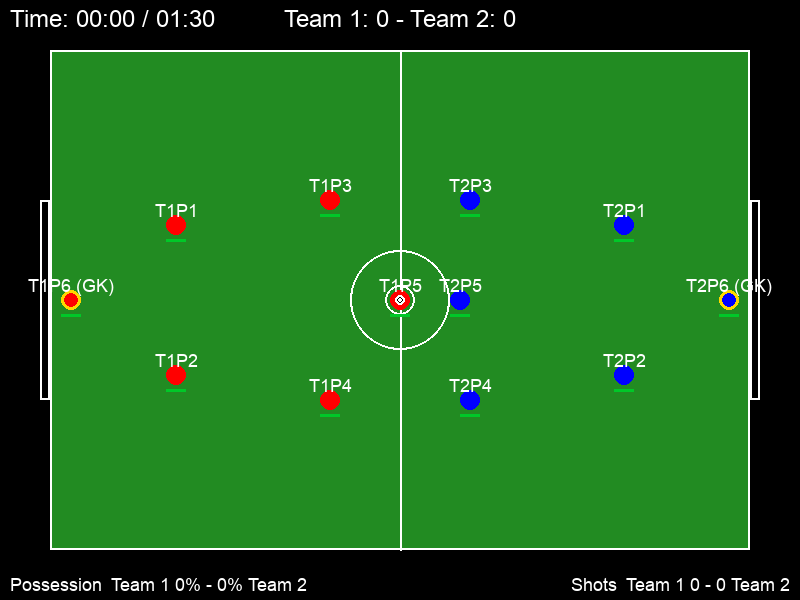
\includegraphics[width=\columnwidth]{kickoff.png}
\caption{Kickoff lineup (t = 0:00). Both teams are clamped into their own
halves in the 2--2--1+GK formation of \cref{tab:formation}; the taker
(T1P5) stands on the centre spot with the ball, and the non-kicking team
respects the centre-circle margin.}
\label{fig:kickoff}
\end{figure}

\begin{figure}[t]
\centering
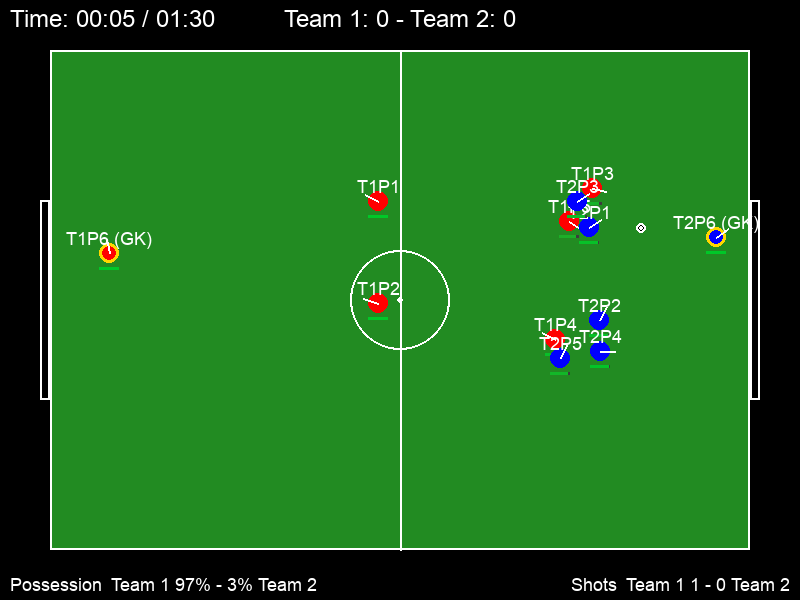
\includegraphics[width=\columnwidth]{defensive_block.png}
\caption{Two-bank defensive block (\cref{eq:block}). With Team~1 (red) out
of possession and the ball far from its goal, its defenders (T1P1, T1P2)
and midfielders (T1P3, T1P4) hold two flat banks whose depth and spacing
track the ball, while the active player presses.}
\label{fig:defblock}
\end{figure}

\begin{figure}[t]
\centering
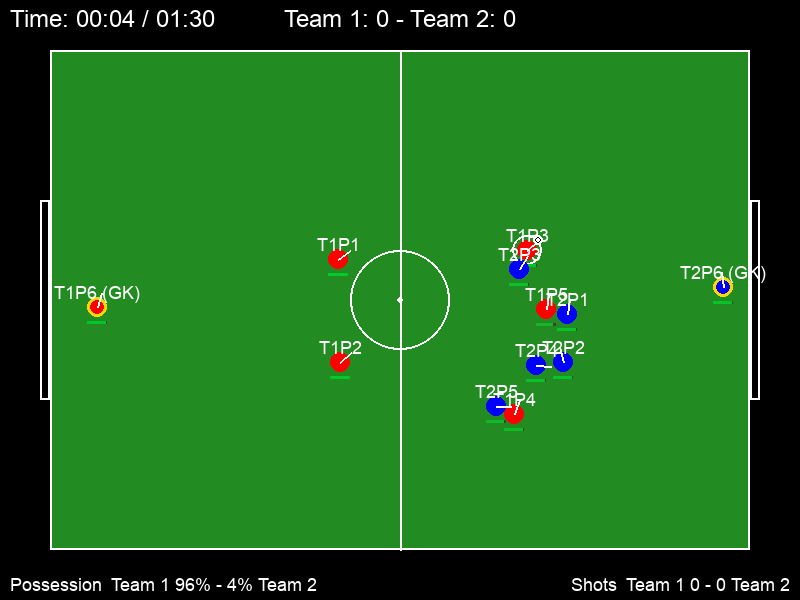
\includegraphics[width=\columnwidth]{man_marking.png}
\caption{Goal-side man-marking (\cref{eq:mark}). The attack has entered
Team~2's threat zone; each blue defender pairs to a red opponent by greedy
nearest-first matching and stations itself $22\px$ goal-side of its man.}
\label{fig:marking}
\end{figure}

\begin{figure}[t]
\centering
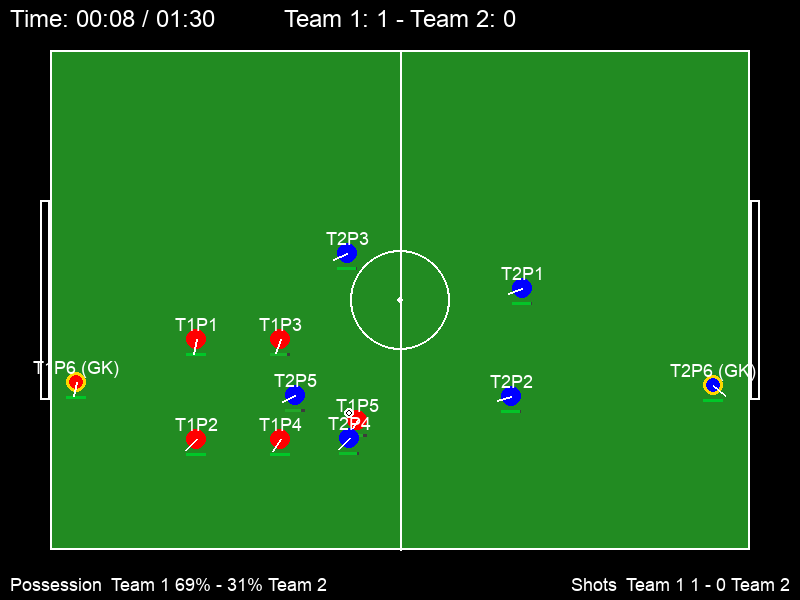
\includegraphics[width=\columnwidth]{rest_defense.png}
\caption{Rest defence (\cref{eq:rest}). While Team~2 (blue) attacks leftward,
its two defenders (T2P1, T2P2) hold a flat cover line to the right of the
ball, so a turnover cannot become an uncontested counter.}
\label{fig:restdef}
\end{figure}

\begin{figure}[t]
\centering
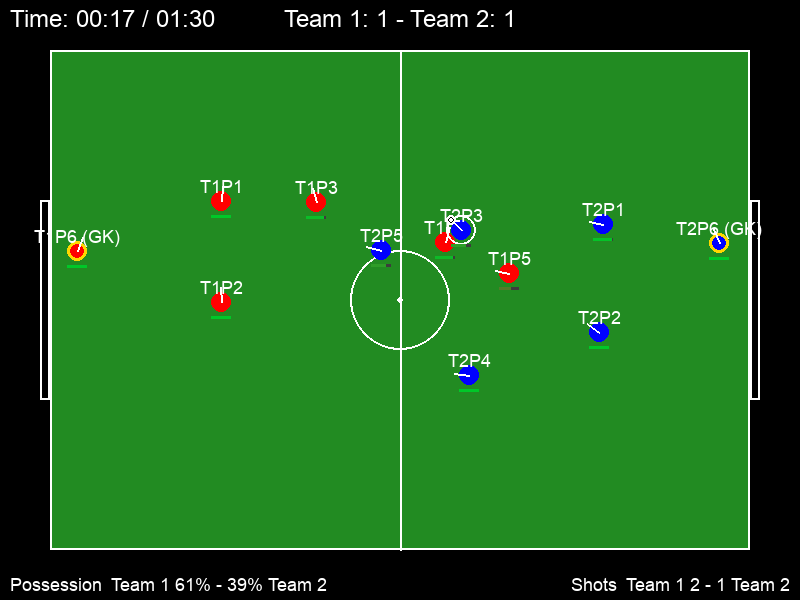
\includegraphics[width=\columnwidth]{attack_support.png}
\caption{Support run (\cref{sec:support}). Team~2's carrier (haloed, near the
halfway line) advances leftward while support runner T2P5 holds a position
ahead of the ball but a buffer inside the offside line, offering the driven
long-ball option.}
\label{fig:support}
\end{figure}

\begin{figure}[t]
\centering
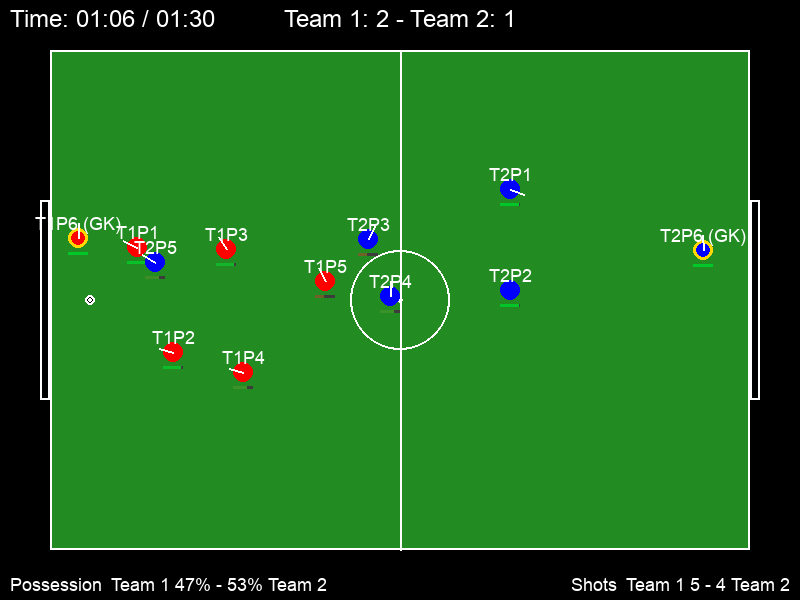
\includegraphics[width=\columnwidth]{goal_line_restart.png}
\caption{Dead-ball restart (\cref{sec:restarts}). The ball left play over
Team~1's goal line off an attacking touch, awarding Team~1 a goal kick
$40\px$ in front of its goal; only the entitled team may collect while
opponents are barred from possession.}
\label{fig:restart}
\end{figure}

\begin{figure}[t]
\centering
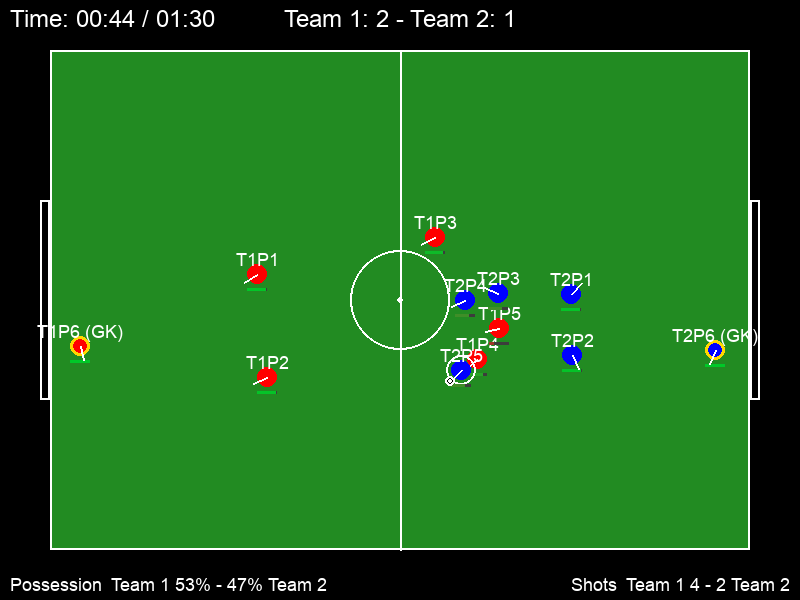
\includegraphics[width=\columnwidth]{midmatch.png}
\caption{Open play at mid-match (t = 0:44, score 2--1). Team shapes remain
distinct: Team~1's defensive structure sits to the left of Team~2's haloed
carrier, the midfield contest is congested, and both keepers hold their lines.}
\label{fig:midmatch}
\end{figure}

% =============================================================================
\section{Experimental Methodology}\label{sec:setup}

\subsection{Headless Harness and Reproducibility}\label{sec:harness}

All experiments run the \emph{unmodified} engine headlessly: SDL is pointed
at a dummy video driver and \code{pygame.time.get\_ticks} is replaced by a
virtual clock advanced by \code{int(1000/60)} = 16~ms per update, so a full
match simulates as fast as the CPU allows while traversing exactly the engine
code paths of the interactive game. This integer-millisecond representation
produces 5{,}625 updates over 90 virtual seconds (an effective 62.5 updates/s);
all frame-rate-sensitive physics and AI probabilities receive the measured
$\Delta t=0.016$~s. The harness constructs
\code{GameEngine(human\_team=None)}, so both sides follow the autonomous
controller path. The mixed-control addition leaves this all-AI path intact;
the full 220-match sweep was rerun after that integration and reproduced the
goal, shot, pass-volume, turnover, ball-flow and shape results. This revision
also corrects the derived definitions of next-possessor pass completion,
held-possession deviation and geometric overlap; runtime was measured again
on the current host. The sweep characterises AI self-play and makes no claim
about human-versus-AI balance or usability.
Python's global PRNG is seeded once per match; every stochastic decision
(tackles, fouls, long shots, offloads, aim noise, kickoff receivers) draws
from this single stream, so a (configuration, seed) pair is fully
reproducible. Instrumentation wraps \code{Player.pass\_ball} to count pass
attempts and completions and samples per-frame state (ball speed,
possession, pairwise distances); the sweep driver overrides module-level
constants between configurations and restores defaults afterwards.

\subsection{Metrics}\label{sec:metrics}

\cref{tab:metrics} defines the per-match metrics. All are computed from
engine state only --- no rendering is involved.

\begin{table}[t]
\centering\small
\begin{threeparttable}
\caption{Per-match metrics recorded by the harness.}
\label{tab:metrics}
\begin{tabular}{@{}p{2.35cm}p{5.35cm}@{}}
\toprule
Metric & Definition \\
\midrule
Goals & total goals by both teams \\
Shots & goal attempts by both teams (keeper clearances excluded) \\
Passes & successful \code{pass\_ball} invocations \\
Pass completion & \% of passes whose next possessor is the intended receiver \\
Possession dev. & $\bigl|\,\text{T1 held-ball share} - 50\%\,\bigr|$ of held-ball time \\
Turnovers & frames on which the holding team changes \\
Free-ball share & \% of frames with no possessor (in-flight, dead or contested balls) \\
Restarts & throw-ins + corners + goal kicks awarded \\
Ball speed & mean over frames with $\lVert\mathbf v_b\rVert > 1\pxs$; stillness = \% of frames $\le 1\pxs$ \\
Spread & mean pairwise distance among Team~1 players, averaged over frames \\
Overlap & \% of frames whose closest player pair is $< 20\px$ apart\tnote{a} \\
\bottomrule
\end{tabular}
\begin{tablenotes}\footnotesize
\item[a] Geometric overlap for two $r_p=10\px$ discs, with a $10^{-6}\px$
tolerance so floating-point contact at $20\px$ is not counted.
\end{tablenotes}
\end{threeparttable}
\end{table}

\subsection{Configurations: Self-Comparison Design}\label{sec:configs}

We sweep five parameters, one at a time, in both directions around the
repository baseline (\cref{tab:configs}), yielding eleven configurations.
Crucially, \emph{both teams always share identical parameters}: every
comparison in \cref{sec:results} is between two configurations of the same
engine playing itself, never between asymmetric opponents. Each
configuration is simulated on the same 20 seeds $\{1,\dots,20\}$
(220 matches in total).

\begin{table}[t]
\centering\small
\caption{Swept configurations. Each varies exactly one constant from the
baseline; both teams always share the same values.}
\label{tab:configs}
\begin{tabular}{@{}llll@{}}
\toprule
Config & Parameter & Value & Baseline \\
\midrule
\textsc{Baseline}      & ---                        & ---   & ---  \\
tackle-low             & $p_{\text{tackle}}$        & 0.01  & 0.05 \\
tackle-high            & $p_{\text{tackle}}$        & 0.15  & 0.05 \\
press-pass-low         & $p_{\text{off}}$           & 0.01  & 0.06 \\
press-pass-high        & $p_{\text{off}}$           & 0.20  & 0.06 \\
long-shot-off          & $p_{\text{long}}$          & 0     & 0.02 \\
long-shot-high         & $p_{\text{long}}$          & 0.10  & 0.02 \\
shoot-short            & $R_{\text{shot}}$          & 100\px & 150\px \\
shoot-long             & $R_{\text{shot}}$          & 220\px & 150\px \\
shape-rigid            & $\kappa_{\text{slide}}$    & 0.2   & 0.5  \\
shape-elastic          & $\kappa_{\text{slide}}$    & 0.8   & 0.5  \\
\bottomrule
\end{tabular}
\end{table}

\subsection{Statistical Protocol}\label{sec:stats}

Configurations share seeds, a common-random-numbers
design~\cite{law2015simulation}: matches with the same seed start from the
identical PRNG stream, and diverge only when a changed parameter first
alters a decision, which removes part of the between-seed variance from
paired contrasts. Each configuration is compared to the baseline on the
paired per-seed differences $d_i = m^{\text{cfg}}_i - m^{\text{base}}_i$
with a two-sided sign-flip permutation test~\cite{good2005permutation}: the
test statistic is $|\bar d|$, and the reference distribution is generated
by $20{,}000$ random sign assignments,
\begin{equation}\label{eq:perm}
p \;=\; \frac{1 + \#\bigl\{\,\pi : \bigl|\overline{\epsilon^{\pi} d}\bigr| \ge |\bar d|\,\bigr\}}{1 + 20\,000},
\qquad \epsilon^{\pi}_i \in \{-1,+1\},
\end{equation}
which is exact under the null of a sign-symmetric paired-difference
distribution and requires no normality assumption. We report effect sizes
(mean paired differences) alongside $p$-values and flag $p<0.05$ ($^{*}$)
and $p<0.01$ ($^{**}$); with 60 contrasts, readers preferring a Bonferroni
posture may use $\alpha = 0.05/60 \approx 0.0008$. We distinguish that
family-wise threshold from the per-contrast markers in the discussion.

% =============================================================================
\section{Results}\label{sec:results}

\subsection{Baseline Characterisation}\label{sec:baseline}

Over 20 seeded matches the baseline produces $7.05 \pm 2.58$ goals,
$14.9 \pm 2.5$ shots and $62.4 \pm 6.6$ passes per 90-second match
(\cref{tab:main}), with held-ball possession $3.9 \pm 2.7$ percentage
points from an even split. Play is continuous: the ball is essentially still
on only $0.8\%$ of frames. Geometric player overlap occurs on
$1.6 \pm 1.3\%$ of frames at the $20\px$ disc-contact threshold, while no
frame crosses the old severe threshold of $15\px$; the pre-rebuild prototype
measured $47.6\%$ stillness and $98.4\%$ severe overlap. The free-ball share
of $43.4\%$ reflects the in-flight windows of kicks, dead-ball restarts and
contested loose balls. Pass completion is $98.1\%$, a direct consequence of
the lane veto (\cref{eq:lane}); we return to this in \cref{sec:discussion}.

\begin{table*}[tp]
\centering\small
\begin{threeparttable}
\caption{Match-production metrics per configuration: mean $\pm$ sd over 20
seeded matches (both teams combined). Possession deviation is the absolute
distance of Team~1's held-ball share from 50\%.}
\label{tab:main}
\begin{tabular}{@{}lcccccc@{}}
\toprule
Config & Goals & Shots & Passes & Pass comp.\ (\%) & Poss.\ dev.\ (pp) & Turnovers \\
\midrule
\SummaryMainRows
\bottomrule
\end{tabular}
\end{threeparttable}
\end{table*}

\begin{table*}[tp]
\centering\small
\caption{Ball-flow and spatial metrics per configuration: mean $\pm$ sd
over 20 seeded matches.}
\label{tab:flow}
\begin{tabular}{@{}lcccccc@{}}
\toprule
Config & Free ball (\%) & Restarts & Ball speed (\pxs) & Still (\%) & Spread (\px) & Overlap (\%) \\
\midrule
\SummaryFlowRows
\bottomrule
\end{tabular}
\end{table*}

\begin{table*}[tp]
\centering\small
\begin{threeparttable}
\caption{Paired self-comparisons against \textsc{Baseline}: mean per-seed
difference ($\Delta$) and sign-flip permutation $p$-value
(\cref{eq:perm}, 20 shared seeds, 20{,}000 resamples).
$^{*}p<0.05$, $^{**}p<0.01$.}
\label{tab:pvalues}
\begin{tabular}{@{}lcccccc@{}}
\toprule
Config & Goals & Shots & Passes & Turnovers & Free ball (pp) & Spread (\px) \\
\midrule
\PValueRows
\bottomrule
\end{tabular}
\end{threeparttable}
\end{table*}

\begin{figure*}[tp]
\centering
\begin{tikzpicture}
\begin{axis}[
  width=0.49\textwidth, height=4.6cm,
  ybar, bar width=5.5pt,
  ymin=0,
  xtick=data,
  xticklabels={Base, $p_t{=}.01$, $p_t{=}.15$, $p_o{=}.01$, $p_o{=}.20$,
               $p_\ell{=}0$, $p_\ell{=}.10$, $R_s{=}100$, $R_s{=}220$,
               $\kappa{=}.2$, $\kappa{=}.8$},
  x tick label style={rotate=45, anchor=east, font=\scriptsize},
  ylabel={goals / match}, ylabel style={font=\small},
  tick label style={font=\scriptsize},
  ymajorgrids, grid style={black!12},
  axis line style={black!60},
]
\addplot+[ybar, fill=barblue, draw=black!60,
  error bars/.cd, y dir=both, y explicit, error bar style={black!70}]
  table[x=idx, y=mean, y error=std] {generated/goals.dat};
\draw[basered, dashed, thick]
  (axis cs:-0.7,7.05) -- (axis cs:10.7,7.05);
\end{axis}
\end{tikzpicture}%
\hfill
\begin{tikzpicture}
\begin{axis}[
  width=0.49\textwidth, height=4.6cm,
  ybar, bar width=5.5pt,
  ymin=0,
  xtick=data,
  xticklabels={Base, $p_t{=}.01$, $p_t{=}.15$, $p_o{=}.01$, $p_o{=}.20$,
               $p_\ell{=}0$, $p_\ell{=}.10$, $R_s{=}100$, $R_s{=}220$,
               $\kappa{=}.2$, $\kappa{=}.8$},
  x tick label style={rotate=45, anchor=east, font=\scriptsize},
  ylabel={shots / match}, ylabel style={font=\small},
  tick label style={font=\scriptsize},
  ymajorgrids, grid style={black!12},
  axis line style={black!60},
]
\addplot+[ybar, fill=barblue, draw=black!60,
  error bars/.cd, y dir=both, y explicit, error bar style={black!70}]
  table[x=idx, y=mean, y error=std] {generated/shots.dat};
\draw[basered, dashed, thick]
  (axis cs:-0.7,14.9) -- (axis cs:10.7,14.9);
\end{axis}
\end{tikzpicture}
\caption{Goal and shot production per configuration (mean $\pm$ sd over 20
seeded matches; dashed line = baseline mean). Removing the long-shot
channel ($p_\ell{=}0$) collapses both; extending the shooting range
($R_s{=}220$) is the only configuration that significantly raises scoring.}
\label{fig:barsgoals}
\end{figure*}

\begin{figure*}[tp]
\centering
\begin{tikzpicture}
\begin{axis}[
  width=0.49\textwidth, height=4.6cm,
  ybar, bar width=5.5pt,
  ymin=0,
  xtick=data,
  xticklabels={Base, $p_t{=}.01$, $p_t{=}.15$, $p_o{=}.01$, $p_o{=}.20$,
               $p_\ell{=}0$, $p_\ell{=}.10$, $R_s{=}100$, $R_s{=}220$,
               $\kappa{=}.2$, $\kappa{=}.8$},
  x tick label style={rotate=45, anchor=east, font=\scriptsize},
  ylabel={passes / match}, ylabel style={font=\small},
  tick label style={font=\scriptsize},
  ymajorgrids, grid style={black!12},
  axis line style={black!60},
]
\addplot+[ybar, fill=barblue, draw=black!60,
  error bars/.cd, y dir=both, y explicit, error bar style={black!70}]
  table[x=idx, y=mean, y error=std] {generated/passes.dat};
\draw[basered, dashed, thick]
  (axis cs:-0.7,62.4) -- (axis cs:10.7,62.4);
\end{axis}
\end{tikzpicture}%
\hfill
\begin{tikzpicture}
\begin{axis}[
  width=0.49\textwidth, height=4.6cm,
  ybar, bar width=5.5pt,
  ymin=0,
  xtick=data,
  xticklabels={Base, $p_t{=}.01$, $p_t{=}.15$, $p_o{=}.01$, $p_o{=}.20$,
               $p_\ell{=}0$, $p_\ell{=}.10$, $R_s{=}100$, $R_s{=}220$,
               $\kappa{=}.2$, $\kappa{=}.8$},
  x tick label style={rotate=45, anchor=east, font=\scriptsize},
  ylabel={turnovers / match}, ylabel style={font=\small},
  tick label style={font=\scriptsize},
  ymajorgrids, grid style={black!12},
  axis line style={black!60},
]
\addplot+[ybar, fill=barblue, draw=black!60,
  error bars/.cd, y dir=both, y explicit, error bar style={black!70}]
  table[x=idx, y=mean, y error=std] {generated/turnovers.dat};
\draw[basered, dashed, thick]
  (axis cs:-0.7,23.4) -- (axis cs:10.7,23.4);
\end{axis}
\end{tikzpicture}
\caption{Circulation metrics per configuration. Passing volume responds
strongly to the offload probability $p_o$ and to formation elasticity
$\kappa$; turnovers scale monotonically with the tackle probability
$p_t$.}
\label{fig:barspasses}
\end{figure*}

\subsection{Possession Contest: Tackle Probability}\label{sec:res-tackle}

$p_{\text{tackle}}$ behaves as a clean dial on duel volatility. Turnovers
scale monotonically: $17.9 \pm 2.0$ at $p_{\text{tackle}}=0.01$,
$23.4 \pm 4.1$ at baseline, $37.1 \pm 6.3$ at $0.15$
(\cref{tab:main,fig:barspasses}); both paired contrasts are significant at
$p < 0.01$ (\cref{tab:pvalues}). Secondary effects are mild and
intuitive: with rare tackles carriers survive longer, take slightly more
shots ($+1.4$, $p=0.032$) and need fewer recycling passes ($-4.1$,
$p=0.043$); goals move within noise in both directions. The contest layer
thus perturbs \emph{who} holds the ball without destabilising the
production chain built on top of it.

\subsection{Pressure Offloading}\label{sec:res-off}

The offload probability $p_{\text{off}}$ governs the dribble-versus-pass
temperament of pressured carriers and produces the largest circulation
swings in the sweep. Passing volume moves from $40.2 \pm 4.5$
($p_{\text{off}}=0.01$, $-22.2$ vs.\ baseline, $p<0.001$) to
$77.4 \pm 7.6$ ($p_{\text{off}}=0.20$, $+15.0$, $p<0.001$). The
free-ball share moves in sympathy ($32.9\%$ vs.\ $48.2\%$): every extra
pass inserts a $\tau_{\text{loose}}$ in-flight window in which nobody
holds the ball. Notably, \emph{eager offloading hurts scoring}: at
$p_{\text{off}}=0.20$ goals drop to $4.15 \pm 1.39$ ($-2.9$,
$p<0.001$) --- pressured carriers who immediately release the ball
(including backward outlets) surrender penetration runs that would
otherwise carry the ball into the long-shot band, while reluctant
offloading ($0.01$) leaves goals statistically unchanged. Individual
ball-carrying, not circulation, is the engine's scoring vector.

\subsection{The Long-Shot Channel}\label{sec:res-long}

The starkest result in the sweep. Setting $p_{\text{long}} = 0$ collapses
shots from $14.9$ to $0.8$ per match and goals from $7.05$ to
$0.85 \pm 0.67$ (both $p < 0.001$): with defenders forming banks, markers
taking goal-side stations and rest defence denying counters, carriers
almost never reach the $R_{\text{shot}} = 150\px$ inner zone with an open
$20^{\circ}$ angle --- in the baseline, \emph{nearly all} goal attempts
originate from the $[150, 320]\px$ long-range band. The defensive stack
is, in other words, highly effective against close-range play, and
long-range strikes are the release valve that keeps matches from
gridlocking. Even the no-long-shot configuration keeps the ball moving
(stillness falls from $0.8\%$ to $0.0\%$), but play concentrates into
sterile midfield circulation, with passes up $+5.7$ and spread up
$+14.8\px$. Raising
$p_{\text{long}}$ to $0.10$ adds $+4.8$ shots ($p<0.001$) but
\emph{no} additional goals ($-0.1$, $p=0.90$): the extra volleys are
lower-quality attempts whose distance-scaled aim noise (\cref{eq:aim})
and the keeper's line-holding absorb the surplus --- a diminishing-returns
profile familiar from real shot-selection analytics.

\subsection{Shooting Range}\label{sec:res-range}

Shrinking the shooting circle to $R_{\text{shot}} = 100\px$ changes
essentially nothing (all $|\Delta|$ small, $p \ge 0.06$): the inner zone
is rarely reached, so its exact radius is immaterial --- consistent with
\cref{sec:res-long}. Extending it to $220\px$ is the only configuration
that significantly \emph{raises} scoring: $8.75 \pm 2.86$ goals
($+1.7$, $p=0.009$) on $+1.7$ shots ($p=0.002$), by converting part of
the probabilistic long-shot band into deterministic first-time attempts.
The asymmetry of the two directions is itself informative: offence in this
engine is gated by \emph{opportunity creation}, not by finishing.

\subsection{Formation Elasticity}\label{sec:res-shape}

The slide gain $\kappa_{\text{slide}}$ trades spatial structure against
local support. The rigid setting ($0.2$) preserves the widest team shape
(spread $198 \pm 4\px$, $+14.3$, $p<0.001$) and yields slightly more
shots ($+2.0$, $p=0.012$) on unchanged goals --- structure suffices,
because the active-player and support-runner mechanisms already deliver
bodies near the ball. The elastic setting ($0.8$) drags all outfield
players toward the ball, shrinking spread ($-4.2\px$) and \emph{reducing}
goals to $4.05 \pm 1.82$ ($-3.0$, $p=0.001$) while inflating passes
($+8.6$, $p<0.001$): congestion around the carrier feeds the openness
term of \cref{eq:passscore} with nearby, marked teammates, producing
sterile short circulation and clogging the very corridors the carrier
would dribble through. Over-concentration is thus actively
counterproductive --- an emergent, rather than programmed, property.

\subsection{Computational Performance}\label{sec:res-perf}

A full 90-second match (5{,}625 16~ms updates, 12 agents) simulates in
$0.760 \pm 0.011$~s of wall-clock time on a single core of an Apple
laptop-class CPU --- $\approx 118\times$ real time, or $7{,}397$
updates/s --- including per-update instrumentation. The entire 220-match
sweep completes in under three minutes, which is what makes the paired
20-seed protocol of \cref{sec:stats} cheap enough to run on every engine
change.

% =============================================================================
\section{Discussion and Limitations}\label{sec:discussion}

\paragraph{What the self-comparison protocol buys.} Because both teams
always share parameters, each contrast in \cref{tab:pvalues} measures the
effect of a mechanism on the \emph{match ecosystem} --- tempo, circulation,
scoring --- rather than on competitive advantage. This is the appropriate
question for engine development: e.g.\ the discovery that
$p_{\text{long}}=0$ gridlocks the game identifies the long-shot channel as
a load-bearing pressure valve, a fact invisible in asymmetric win-rate
testing where both sides would lose it simultaneously. The paired
common-random-numbers design sharpens these contrasts at zero extra
simulation cost, although its variance-reduction benefit decays over the
match horizon: a single divergent tackle roll desynchronises subsequent
draws from the shared stream, so late-match state decorrelates between
paired runs.

\paragraph{Validity of magnitudes.} Match statistics are stylised rather
than calibrated to real football: 90 simulated seconds, six-a-side, a
scoring rate of $\sim$7 goals per match, and a 98\% pass completion rate.
The completion figure exposes a modelling gap --- opponents do not
\emph{anticipate} passes (no interception behaviour beyond standing in the
lane at kick time), so the lane veto (\cref{eq:lane}) is nearly
sufficient for success. Adding reactive interception would lower
completion and likely amplify the cost of eager offloading found in
\cref{sec:res-off}.

\paragraph{Numerical and geometric approximations.} Exponential velocity
attenuation and movement-command blending are timestep-corrected, but the
drift-then-decay position update retains finite-step error. The shot-angle
policy also uses an unwrapped absolute \code{atan2} difference
(\cref{eq:angle}), so geometrically mirrored positions can receive different
values. These implementation details are part of the evaluated baseline,
rather than properties of an ideal continuous or perfectly mirrored model.

\paragraph{Perception and fairness.} Perception is perfect, global and
symmetric; there is no sensor noise, unlike the RoboCup
server~\cite{chen2003manual}. Fairness between the mirrored AI teams is
enforced structurally (central possession contest, controller commands
issued before integration) and reflected by configuration-level mean
held-possession deviations of $2.1$--$3.9$~pp in \cref{tab:main}.
Mixed-control mode preserves
the same physical and rules-level fairness: input cannot assign possession,
and human actions use the same kick, stamina and cooldown methods. It does
not claim decision-policy symmetry --- AI passes receive lane and offside
filtering while human passes use the facing-cone heuristic of
\cref{sec:human}.

\paragraph{Mixed-control evaluation scope.} The interactive path is covered
by deterministic tests of input semantics, player selection, AI exclusion,
on-ball actions, visual markers and rules invariants, but it is absent from
the 220-match parameter sweep. No user study, win-rate calibration or
human-versus-AI difficulty evaluation has yet been performed. The all-AI
results should therefore be read as a characterisation of the simulation
substrate and autonomous policy, not as evidence that the interactive match
is competitively balanced.

\paragraph{Threats to inference.} The sign-flip test is exact under
sign-symmetry of paired differences, but seeds induce heavy-tailed match
outcomes (goal counts are small integers); we therefore emphasise effects
that are large, monotone across the swept direction, and significant at
$p<0.01$. The long-shot removal, eager-offload and turnover effects survive a
Bonferroni correction across the 60 contrasts
($\alpha\approx0.0008$). The high-elasticity scoring effect remains
significant at the stated $p<0.01$ level ($p\approx0.0015$) but does not cross
that family-wise threshold.

% =============================================================================
\section{Conclusions and Future Work}\label{sec:conclusion}

This paper specified, end to end, the methodology of the Futebole 2D
soccer simulation: timestep-aware point-mass physics with
range-inverted kick powers (\cref{eq:reach,eq:passpower,eq:shotpower}),
an order-independent probabilistic possession contest with fouls and
entitled restarts (\cref{alg:possession}), and a layered tactical model
--- elastic formations, two-bank blocks, goal-side marking, rest defence,
veto-based decision passing and angle-gated noisy shooting --- each
specified by explicit equations and algorithms and illustrated with frames
from the running simulation. The same engine now supports interactive
mixed control: a semantic input layer drives one phase-selected
player, the tactical AI coordinates the remaining teammates, and an explicit
exclusion boundary prevents both controllers from commanding the same
player while preserving the central rules.

A paired, seeded parameter sweep evaluated the engine strictly against
itself. Three findings stand out: (i)~the long-range shooting channel is
the dominant scoring mechanism --- removing it reduces scoring by 88\%
and reveals that the defensive stack effectively seals the close-range
game; (ii)~individual ball-carrying outperforms eager circulation ---
raising the pressured-offload rate or the formation's attraction to the
ball each cut scoring by $\sim$40\% with high significance; and (iii)~the
tackle probability provides a well-behaved, monotone control over duel
volatility without side effects on production. At $118\times$ real time,
the full statistical protocol is cheap enough to serve as a regression
harness for every future engine change.

Future work follows the repository's tactical backlog: explicit
counter-attack and recovery transitions, width preservation and crossing,
multiple coordinated off-ball runs, structured build-up from goal kicks, a
team pressing model with triggers, penalty-box organisation, set-piece
shapes, and score/clock-aware tempo management, followed by scaling toward
11-a-side rosters. For mixed control, the next steps are human-versus-AI
playtesting and difficulty calibration, lane-aware assisted targeting,
engine-level offside enforcement shared by both control modes, and explicit
goalkeeper-control and defensive-selection options. On the evaluation side,
reactive pass interception
and a calibration pass mapping simulated rates onto real-football
distributions are the natural next steps, as is porting the
strategy-recommendation layer of~\cite{abreu2014improving} onto Futebole
as a testbed --- with the parametric self-comparison protocol of
\cref{sec:setup} serving as the control condition.

% =============================================================================
\begin{thebibliography}{12}\footnotesize

\bibitem{kitano1997robocup}
H.~Kitano, M.~Asada, Y.~Kuniyoshi, I.~Noda, E.~Osawa,
RoboCup: the robot world cup initiative,
in: Proceedings of the First International Conference on Autonomous
Agents, ACM, 1997, pp.~340--347.

\bibitem{chen2003manual}
M.~Chen, K.~Dorer, E.~Foroughi, et al.,
Users Manual: RoboCup Soccer Server for Soccer Server Version 7.07 and
Later, The RoboCup Federation, 2003.

\bibitem{abreu2014improving}
P.~Henriques Abreu, D.~Castro Silva, F.~Almeida, J.~Mendes-Moreira,
Improving a simulated soccer team's performance through a Memory-Based
Collaborative Filtering approach,
Applied Soft Computing 23 (2014) 180--193.

\bibitem{akiyama2008positioning}
H.~Akiyama, I.~Noda,
Multi-agent positioning mechanism in the dynamic environment,
in: RoboCup 2007: Robot Soccer World Cup XI, Springer, 2008, pp.~377--384.

\bibitem{stone2000multiagent}
P.~Stone, M.~Veloso,
Multiagent systems: a survey from a machine learning perspective,
Autonomous Robots 8 (3) (2000) 345--383.

\bibitem{reynolds1999steering}
C.~W. Reynolds,
Steering behaviors for autonomous characters,
in: Proceedings of the Game Developers Conference, 1999, pp.~763--782.

\bibitem{law2015simulation}
A.~M. Law,
Simulation Modeling and Analysis, 5th ed., McGraw-Hill, New York, 2015.

\bibitem{good2005permutation}
P.~Good,
Permutation, Parametric and Bootstrap Tests of Hypotheses, 3rd ed.,
Springer, New York, 2005.

\bibitem{demsar2006statistical}
J.~Dem\v{s}ar,
Statistical comparisons of classifiers over multiple data sets,
Journal of Machine Learning Research 7 (2006) 1--30.

\bibitem{shinners2011pygame}
P.~Shinners,
Pygame: Python game development library, version 2.5.2,
\url{https://www.pygame.org}, 2011 (accessed 2026).

\end{thebibliography}

\end{document}
